\section{Auswertung}
\label{sec:Auswertung}
\subsection{Bestimmung der maximalen Feldstärke}
Um die maximale Feldstärke zu bestimmen, wird eine Hallsonde entlang der $z$-Achse verschoben und die damit gemessene 
Feldstärke wird notiert.
Die Messwerte sind in Tablle \ref{tab:Feldstärke} augelistet.
\FloatBarrier
\begin{table}
  \centering
  \begin{tabular}{c c}
    \toprule
    $z$ / \SI{}{\milli\meter}& $B$ / \SI{}{\milli\tesla}\\
    \midrule
    125& 202\\     
    123& 298\\
    121& 359\\
    119& 389\\
    117& 404\\
    116& 406\\
    115& 410\\
    114& 409\\
    113& 409\\
    111& 402\\
    109& 386\\
    107& 355\\
    \bottomrule
  \end{tabular}
  \caption{Messwerte zur Bestimmung der maximalen Feldstärke.}
  \label{tab:Feldstärke}
\end{table}
\FloatBarrier
Die Werte aus der Tablle \ref{tab:Feldstärke} werden in Abbildung \ref{fig:Feldstärke} dargestellt.
\FloatBarrier
\begin{figure}
  \centering
  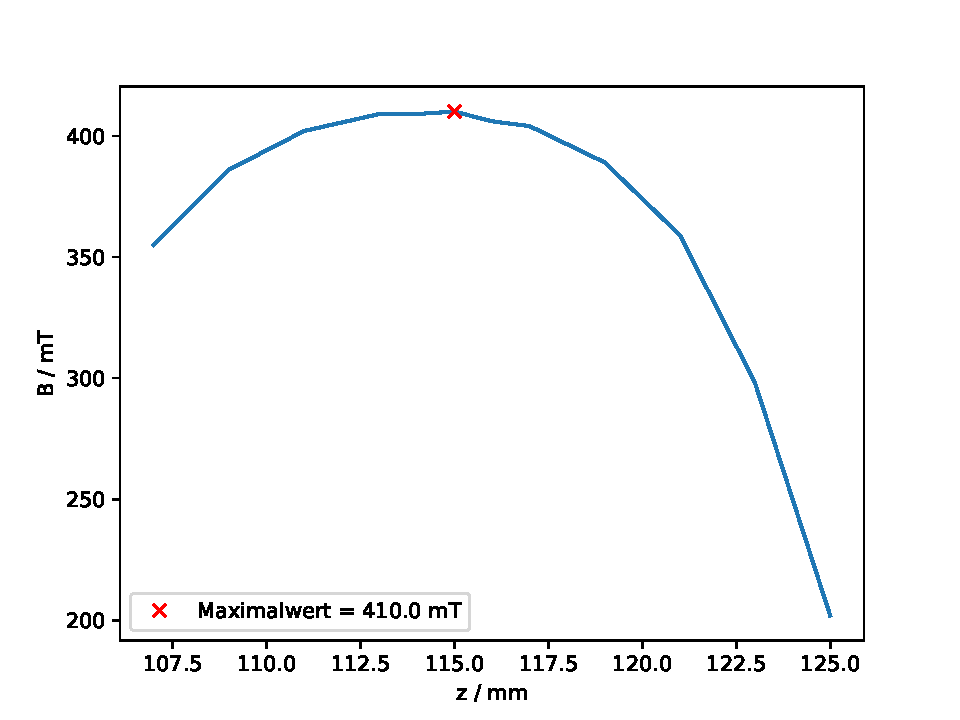
\includegraphics[width = \textwidth, keepaspectratio]{figure/BFeld_plot.pdf}
  \caption{Graphische Darstellung der Messwerte für die Bestimmung der maximalen Feldstärke.}
  \label{fig:Feldstärke}
\end{figure}
\FloatBarrier
Der Maximale Wert liegt bei \SI{410}{\milli\tesla}. 
\subsection{Bestimmung der effektiven Masse}
Für die Bestimmung der effektiven Masse wird der Drehwinkel der Polarisationsebene in Abhängigkeit der Wellenlänge gemessen.
Diese Daten werden für zwei n-dotierte und eine reine Probe aufgenommen. Da die Proben unterschiedlich dick sind, wird 
der Drehwinkel auf die Dicke der Probe normiert.
Die Messwerte sind in Tablle \ref{tab:Drehwinkel} notiert.
\FloatBarrier
\begin{table}
  \centering
  \begin{tabular}{c c c c}
    \toprule
    $\lambda$ / \SI{}{\micro\meter}& $\theta_{\text{n-dotiert 1}}$ / $\frac{\SI{}{\radian}}{\SI{}{\micro\meter}}$& 
    $\theta_{\text{n-dotiert 2}}$ / $\frac{\SI{}{\radian}}{\SI{}{\micro\meter}}$&
    $\theta_{\text{rein}}$ / $\frac{\SI{}{\radian}}{\SI{}{\micro\meter}}$\\
    \midrule
    $\num{1.06} $&$\num{3.85e-4}$&$\num{1.57e-4}$&$\num{0.80e-4}$\\
    $\num{1.29} $&$\num{2.02e-4}$&$\num{1.25e-4}$&$\num{0.59e-4}$\\
    $\num{1.45} $&$\num{0.41e-4}$&$\num{1.22e-4}$&$\num{0.45e-4}$\\
    $\num{1.72} $&$\num{0.42e-4}$&$\num{1.31e-4}$&$\num{0.34e-4}$\\
    $\num{1.96} $&$\num{1.27e-4}$&$\num{1.45e-4}$&$\num{0.24e-4}$\\
    $\num{2.156}$&$\num{0.96e-4}$&$\num{1.63e-4}$&$\num{0.19e-4}$\\
    $\num{2.34} $&$\num{1.64e-4}$&$\num{1.75e-4}$&$\num{0.17e-4}$\\
    $\num{2.51} $&$\num{3.54e-4}$&$\num{2.05e-4}$&$\num{0.12e-4}$\\
    $\num{2.65} $&$\num{1.09e-4}$&$\num{1.84e-4}$&$\num{0.19e-4}$\\
    \bottomrule
  \end{tabular}
  \caption{Normierter Drehwinkel in Abhängigkeit der Wellenlänge. Die Dicken der Probe sind: Probe 1 $d=\SI{1360}{\micro\meter}$,
  Probe 2 $d=\SI{1296}{\micro\meter}$, reine Probe $d=\SI{5110}{\micro\meter}$.}
  \label{tab:Drehwinkel}
\end{table}
\FloatBarrier
